\section{Controladores PID}


\begin{frame}{Cálculo diferencial e integral}
	\begin{block}{Introdução}
		\begin{itemize}
			\item O cálculo diferencial e integral é uma das disciplinas \textbf{mais estudadas e usadas em todo o mundo}, devido a sua \textbf{utilidade}.
			\item Todo o cálculo se baseia no conceito fundamental do \textbf{limite}, que é uma operação matemática de análise de \textbf{tendência}.
		\end{itemize}
	\end{block}
\end{frame}


\begin{frame}{Cálculo diferencial e integral}
	\begin{block}{Limites - Exemplo \#01}
		\begin{itemize}
			\item Por exemplo: qual a tendência da função $ f(x)=\dfrac{x}{2} $ quando $ x $ se aproxima de $ 2 $?
		\end{itemize}
	\end{block}
	
%	\smallskip
	
	\centering
	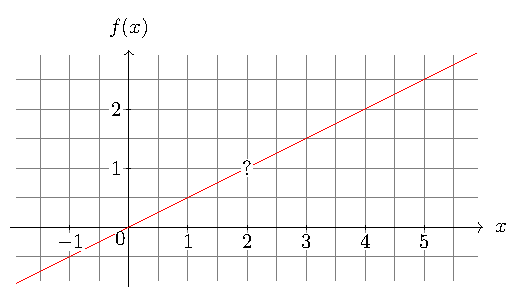
\includegraphics[width=0.8\linewidth]{Figuras/Ch13/lim1}
\end{frame}


\begin{frame}{Cálculo diferencial e integral}
	\begin{block}{Limites - Exemplo \#01}
		\begin{itemize}
			\item A mesma pergunta, no cálculo, é o limite de $ x/2 $ com $ x $ tendendo a $ 2 $, ou:\[ \lim\limits_{x\to 2}\dfrac{x}{2} \]
			
		\end{itemize}
	\end{block}
	
%	\smallskip
	
	\centering
	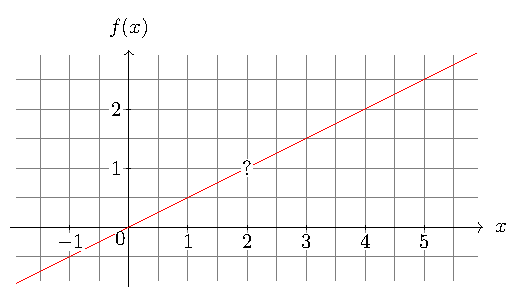
\includegraphics[width=0.8\linewidth]{Figuras/Ch13/lim1}
\end{frame}


\begin{frame}{Cálculo diferencial e integral}
	\begin{block}{Derivadas e integrais - introdução}
		\begin{itemize}
			\item A partir desse conceito, podemos definir outras ideias mais interessantes, como as \textbf{derivadas} e \textbf{integrais}.
			\item As derivadas lidam com a \textbf{taxa de variação} de algo perto de zero, ou seja, para uma \textbf{mudança minúscula em} $ \bm{x} $, quanto vai se alterar $ \bm{f(x)} $? (pense numa função)
			\[ \dfrac{\dif}{\dif x}\sbr{f(x)} \]
			\item Já a integral lida com a \textbf{área} de uma função em relação a um \textbf{eixo}, ou seja, de tal ($ a $) valor a tal ($ b $) valor, qual a \textbf{área entre a linha da função e o eixo} $ \bm{x} $?
			\[ \int_{a}^{b}f(x)\dif x \]
		\end{itemize}
	\end{block}
\end{frame}


\begin{frame}{Cálculo diferencial e integral}
	\begin{block}{Derivada gráfica}
		\begin{itemize}
			\item A derivada pode ser visualizada como a \textbf{reta tangente à linha da função} no gráfico.
		\end{itemize}
	\end{block}

	\centering
	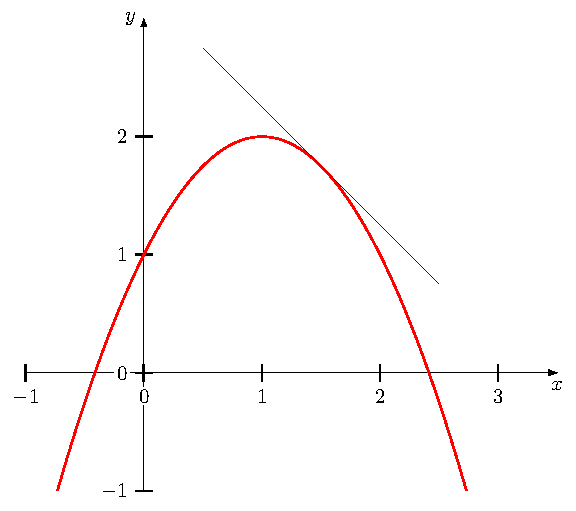
\includegraphics[width=0.5\linewidth]{Figuras/Ch13/der2}

\end{frame}


\begin{frame}{Cálculo diferencial e integral}
	\begin{block}{Integral gráfica}
		\begin{itemize}
			\item A integral pode ser visualizada como a \textbf{área entre a curva e o eixo} $ \bm{x} $.
		\end{itemize}
	\end{block}

	\centering
	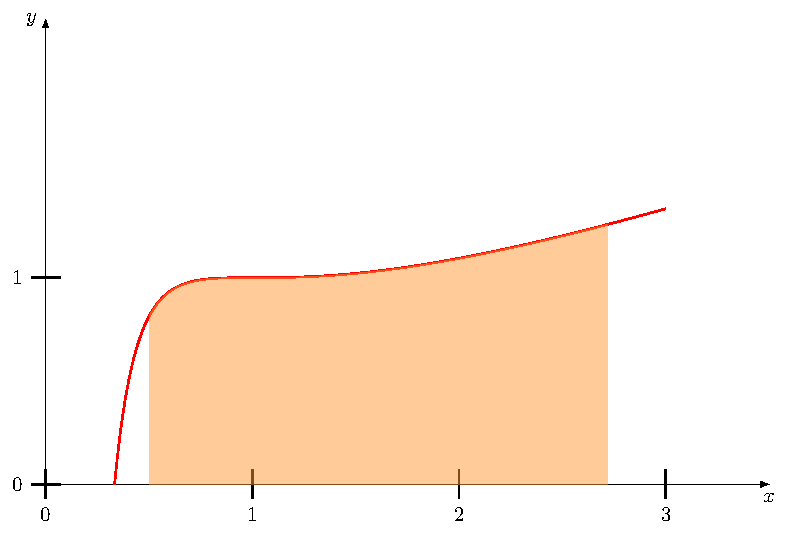
\includegraphics[width=0.7\linewidth]{Figuras/Ch13/int2}
	
\end{frame}


\begin{frame}{Cálculo diferencial e integral}
	\begin{block}{Integral e derivada - Definição limitante}
		Essas abordagens se baseiam em tendências, respectivamente:
		\begin{itemize}
			\item A tendência de $ \bm{\dfrac{\Delta y}{\Delta x}} $ conforme os \textbf{deltas} (intervalos) \textbf{tendem a zero}.
			\item A tendência da \textbf{soma de retângulos} de bases iguais e alturas que tocam no gráfico conforme suas \textbf{bases tendem a zero}.
		\end{itemize}
	\end{block}
\end{frame}


\begin{frame}{Cálculo diferencial e integral}
	\begin{minipage}{0.49\linewidth}
		\centering
		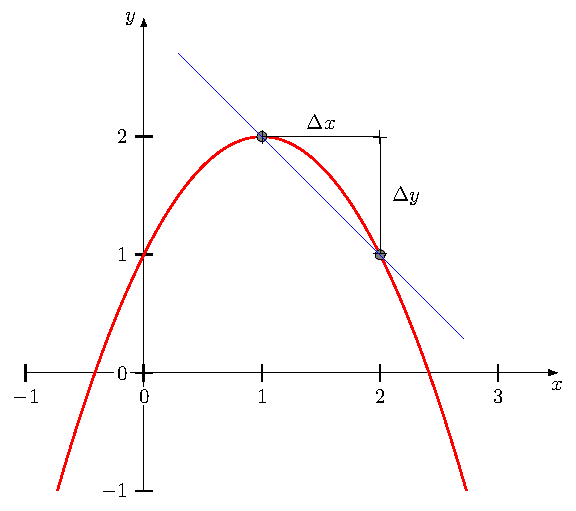
\includegraphics[width=1\linewidth]{Figuras/Ch13/der1}
	\end{minipage}\tikzmark{p1}
	\hfill
	\begin{minipage}{0.49\linewidth}
		\centering
		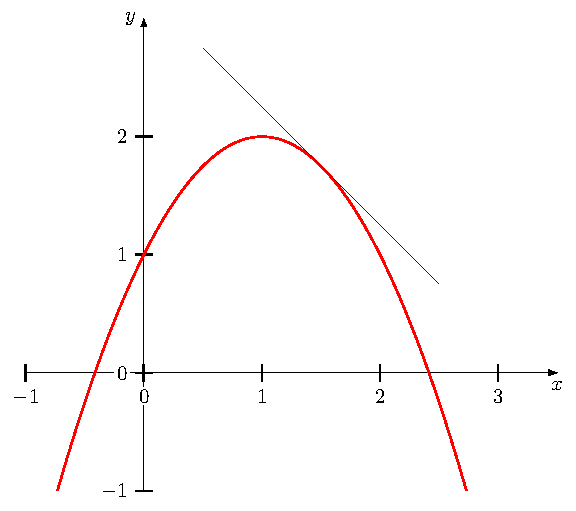
\includegraphics[width=1\linewidth]{Figuras/Ch13/der2}
	\end{minipage}
	
	\begin{tikzpicture}[overlay, remember picture]
		\draw[-Implies, double distance=2pt,thick] (p1) ++(-0.3cm,0) -- +(1,0);
	\end{tikzpicture}
\end{frame}


\begin{frame}{Cálculo diferencial e integral}
	\begin{minipage}{0.49\linewidth}
		\centering
		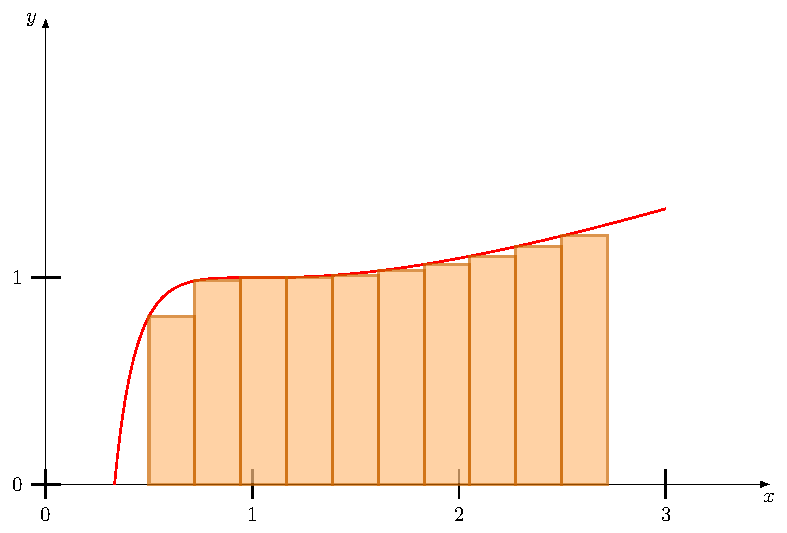
\includegraphics[width=1\linewidth]{Figuras/Ch13/int1}
	\end{minipage}\tikzmark{p1}
	\hfill
	\begin{minipage}{0.49\linewidth}
		\centering
		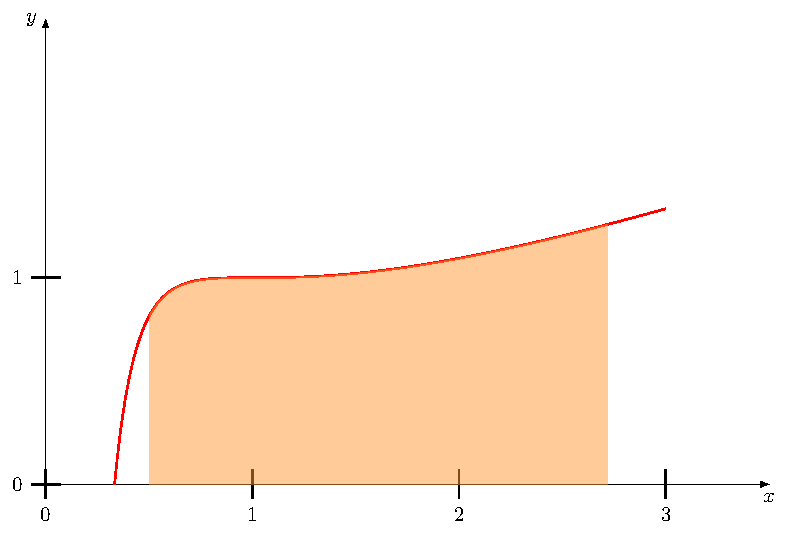
\includegraphics[width=1\linewidth]{Figuras/Ch13/int2}
	\end{minipage}
	
	\begin{tikzpicture}[overlay, remember picture]
	\draw[-Implies, double distance=2pt,thick] (p1) ++(-0.8cm,0) -- +(1,0);
	\end{tikzpicture}
\end{frame}


\begin{frame}{Cálculo diferencial e integral}
	\begin{block}{Monômios - Introdução e derivada}
		\begin{itemize}
			\item Os monômios são os \textbf{primeiros casos} de derivação e integração que são ensinados, já que possuem regras \textbf{fáceis de aplicar e lembrar}.
			\item Um monômio é uma expressão no formato $ a\cdot x^{n} $, com $ n\in\set{0,1,2,3,\ldots} $.
			\item A derivação é uma operação \textbf{mais fácil} do que a integração e, por isso, aprendemos ela primeiro.
			\item A \textbf{derivada} de um monômio \[  m(x)=a\cdot x^{n} \] será igual a \[ \od{m(x)}{x}= a n\cdot x^{n-1} \]
		\end{itemize}
	\end{block}
\end{frame}


\begin{frame}{Cálculo diferencial e integral}
	\begin{block}{Regra da potência - Exemplo \#01}
		\begin{itemize}
			\item Como é possível notar, a derivada de um monômio segue uma regra relativa ao seu \textbf{expoente}, onde ele simplesmente \textbf{``cai para frente''}, subtraindo um do expoente.
			\item Por exemplo, a derivada de $ 3x^{2} $ é \[ \diff{}{x}\sbr{3x^{2}} =3\cdot2x^{2-1}=6x  \]
			\item Essa regra é conhecida como \textbf{``regra da potência''}.
		\end{itemize}
	\end{block}
\end{frame}


\begin{frame}{Cálculo diferencial e integral}
	\begin{block}{Derivação de polinômios - Exemplo \#01}
		\begin{itemize}
			\item Um \textbf{polinômio} é uma expressão formada por \textbf{monômios}, todos \textbf{somados}.
			\item Um exemplo de polinômio seria $ p(x)=12x^{3}+3x^{2} $.
			\item Para \textbf{derivar um polinômio} podemos simplesmente aplicar a regra da potência a \textbf{cada termo} e \textbf{somar os resultados} ao final, por exemplo:
			\[ \diff{}{x}\sbr{x^{3}+2x}=\diff{}{x}\sbr{x^{3}}+\diff{}{x}\sbr{2x}=3x^{3-1}+2\cdot 1x^{1-1}=3x^{2}+2 \]
		\end{itemize}
	\end{block}
\end{frame}


\begin{frame}{Cálculo diferencial e integral}
	\begin{block}{Regra da potência - Propriedades}
		É importante notar algumas propriedades dos monômios sob a derivação:
		\begin{enumerate}
			\item \[ \diff{}{x}\sbr{ax^{n}}=a\diff{}{x}\sbr{x^{n}} \]
			\item \[ \diff{}{x}\sbr{ax^{0}}=\diff{}{x}\sbr{a}=0 \]
		\end{enumerate}
		Sendo assim, dizemos que a \textbf{derivada de uma constante} é \textbf{sempre} $ \bm{0} $.
	\end{block}
\end{frame}


%\begin{frame}{Cálculo diferencial e integral}
%	\begin{block}{Derivação implícita - Regra da cadeia}
%		\begin{itemize}
%			\item Em todo caso onde temos \textbf{mais de uma variável} em uma expressão, vale notar que a derivação deve ser feita \textbf{com respeito à variável no operador}.
%			\item Mas qualquer outra variável que apareça pode ser derivada \textbf{implicitamente}, ou seja, \textbf{sem alterar a expressão}.
%			\item No caso de uma única variável, podemos utilizar a \textbf{``regra da cadeia''}, que enuncia que podemos realizar \textbf{operações intermediárias} em função de \textbf{variáveis auxiliares}.
%		\end{itemize}
%	\end{block}
%\end{frame}


%\begin{frame}{Cálculo diferencial e integral}
%	\begin{block}{Derivação implícita - Exemplos \#01 e \#02}
%		\begin{itemize}
%			\item Derivando $ y $ em relação a $ x $ temos:
%			\begin{align*}
%				\diff{}{x}\sbr{y}&=\left( \diff{y}{x}\diff{}{y}\right) \sbr{y}\\
%								 &=\diff{y}{x}\left( \diff{}{y}\sbr{y}\right)\\
%								 &=\diff{y}{x}(1)=\od{y}{x}
%			\end{align*}
%			\item No caso ilustrado, como não era possível derivar $ \bm{y} $ em relação a $ \bm{x} $, \textbf{``separamos'' a derivada} de $ y $ em relação a $ x $ e abrimos \textbf{outra derivada} em relação ao próprio $ y $, sob a qual a operação poderia ser realizada.
%			\item Derivando $ 10z $ em relação a $ y $ temos:
%			\[ \diff{}{y}\sbr{10z^{2}}=\diff{z}{y}\diff{}{z}\sbr{10z^{2}}=\diff{z}{y}10\cdot2z=20z \]
%		\end{itemize}
%	\end{block}
%\end{frame}


%\begin{frame}{Cálculo diferencial e integral}
%	\begin{block}{Regra da cadeia}
%		\begin{itemize}
%			\item É possível generalizar mais a regra de cadeia para além do caso mostrado, como, por exemplo, para funções compostas $ f\circ g=f(g(x)) $.
%			\item Um exemplo de composta seria $ \sqrt{x^{2}-1} $, onde $ f(x)=\sqrt{x} $ e $ g(x)=x^{2}-1 $, portanto, $ f(g(x))=\sqrt{g(x)}=\sqrt{x^{2}-1} $.
%			\item Sua derivada é:
%			\[ \diff{}{x}\sbr{f(g(x))}=\diff{f(u)}{u}\diff{}{x} \]
%		\end{itemize}
%	\end{block}
%\end{frame}


\begin{frame}{Cálculo diferencial e integral}
	\begin{block}{Integração de monômios - Teorema fundamental do cálculo}
		\begin{itemize}
			\item O \textbf{teorema fundamental do cálculo} estabelece, em termos simples, que para toda função derivada, podemos \textbf{retornar à original} integrando-a.
			\item Esse teorema estabelece, basicamente, que a \textbf{derivação} e a \textbf{integração} são \textbf{operações contrárias}, assim como a multiplicação e a divisão.
			\item Desta forma, existe uma função $ f(x) $ para a qual \[ \int \od{f(x)}{x} \dif x=f(x) \]
			\item Sendo assim, dado um monômio $ m(x)=a\cdot x^{n} $, podemos integrá-lo aplicando a regra da potência ao contrário, ou seja:
			\[ \int a\cdot x^{n} \dif x=\dfrac{a \cdot x^{n+1}}{(n+1)} \]
		\end{itemize}
	\end{block}
\end{frame}


\begin{frame}{Cálculo diferencial e integral}
	\begin{block}{Integração de monômios - Exemplo \#01}
		\begin{itemize}
			\item Para exemplificar esse teorema, podemos derivar e integrar qualquer monômio, por exemplo:
			\[ m(x)=2x^{5} \]
			Derivando, temos:
			\[ \od{m(x)}{x}=2\cdot 5 x^{5-1}=10x^{4} \]
			Integrando, devemos retornar a $ p(x) $:
			\[ \int 10x^{4} \dif x=\dfrac{10x^{4+1}}{4+1}=\dfrac{10x^{5}}{5}=2x^{5} \]
		\end{itemize}
	\end{block}
\end{frame}


\begin{frame}{Cálculo diferencial e integral}
	\begin{block}{Integração de polinômios - Exemplo \#01}
		\begin{itemize}
			\item Da mesma forma que podemos \textbf{somar as derivadas} de cada parte de um polinômio, também podemos \textbf{somar as integrais}, por exemplo:
			\[ \int x^{3}+2x \dif x=\int x^{3} \dif x + \int 2x \dif x= \dfrac{x^{3+1}}{3+1}+\dfrac{2x^{1+1}}{1+1}=\dfrac{x^{4}}{4}+x^{2} \]
		\end{itemize}
	\end{block}
\end{frame}


\begin{frame}{Cálculo diferencial e integral}
	\begin{block}{Integral definida - Introdução}
		\begin{itemize}
			\item A integral, geralmente, é aplicada só a um \textbf{determinado trecho de uma função}, e não de forma pura (indefinida), como vimos até agora.
			\item A \textbf{integral definida} $ \displaystyle\int_{a}^{b}p(x) \dif x $ é definida como \[ \eval{\left( \int f(x) \dif x\right) }_{a}^{b}=\int f(b) \dif x-\int f(a) \dif x \]
			que é, basicamente, a \textbf{diferença entre dois pontos} da função integrada, ou, a \textbf{área sob a curva} de uma \textbf{parte} da função que integramos.
		\end{itemize}
	\end{block}
\end{frame}


\begin{frame}{Cálculo diferencial e integral}
	\begin{block}{Integral definida - Exemplo \#01}
		\begin{itemize}
			\item A \textbf{integral definida} de $ f(x)=x^{2} $ entre $ 2 $ e $ 5 $ pode ser calculada por:
			\begin{align*}
			\int_{2}^{5}x^{2}\dif x&=\eval{\left( \dfrac{x^{3}}{3}\right) }_{2}^{5}=\\[0.5em]
			&=5^{3}-2^{3}=\\
			&=125-8=\boxed{117}
			\end{align*}
		\end{itemize}
	\end{block}
\end{frame}


\begin{frame}{Cálculo diferencial e integral}
	\begin{block}{Integral definida e indefinida - Exemplo \#02}
		\begin{itemize}
			\item Levando em conta que toda \textbf{derivação de uma constante} vai torná-la \textbf{nula}, sempre que realizamos uma operação de \textbf{integral indefinida}, devemos adicionar uma \textbf{constante} $ \bm{C} $, que faz o papel dessa constante \textbf{perdida} na derivação.
			\item Por exemplo:\[ \int 3x^{2} \dif x=\dfrac{3x^{3}}{3} + C=x^{3}+C \]
		\end{itemize}
	\end{block}
\end{frame}


\begin{frame}{Cálculo diferencial e integral}
	\begin{block}{Revisão}
		01. Realize as seguintes operações:
		
		\smallskip
		
		\begin{minipage}{0.49\linewidth}
			(a) $ \diff{}{x}\sbr{x} $
			
			\vspace{0.5cm}
			
			(b) $ \diff{}{x}\sbr{3x^{2}} $
			
			\vspace{0.5cm}
			
			(c) $ \diff{}{x}\sbr{x^{3}+2x} $
			
			\vspace{0.5cm}
			
			(d) $ \diff{}{x}\sbr{3x^{2}-x} $
		\end{minipage}
		\hfill
		\begin{minipage}{0.49\linewidth}
			(e) $ \diff{}{x}\sbr{4x+2x^{2}} $
			
			\vspace{0.5cm}
			
			(f) $ \diff{}{y}\sbr{4y+3y^{2}} $
			
			\vspace{0.5cm}
			
			(g) $ \diff{}{x}\sbr{x^{-1}} $
			
			\vspace{0.5cm}
			
			(h) $ \diff{}{x}\sbr{\dfrac{2}{x}+3x^{2}} $
		\end{minipage}
	\end{block}
\end{frame}


\begin{frame}{Cálculo diferencial e integral}
	\begin{block}{Revisão}
		02. Realize as seguintes operações:
		
		\smallskip
		
		\begin{minipage}{0.49\linewidth}
			(a) $ \displaystyle\int x \dif x $
			
			\vspace{0.5cm}
			
			(b) $ \displaystyle\int x^{2} \dif x $
			
			\vspace{0.5cm}
			
			(c) $ \displaystyle\int x^{3}+3x \dif x $
			
			\vspace{0.5cm}
			
			(d) $ \displaystyle\int 2x+3x^{2}+4x^{3}\dif x $
		\end{minipage}
		\hfill
		\begin{minipage}{0.49\linewidth}
			(e) $ \displaystyle\int \dif x $
			
			\vspace{0.5cm}
			
			(f) $ \displaystyle\int y+2y^{2} \dif y $
			
			\vspace{0.5cm}
			
			(g) $ \displaystyle\int x^{2}-3x^{3} \dif x $
			
			\vspace{0.5cm}
			
			(h) $ \displaystyle\int x^{3}+2x^{2} \dif x $
		\end{minipage}
	\end{block}
\end{frame}


\begin{frame}{Cálculo diferencial e integral}
	\begin{block}{Revisão}
		03. Refaça todas as integrais indefinidas do exercício anterior como definidas entre $ 0 $ e $ 3 $.
		
		\vspace{1cm}
		
		04. Resolva: \[ \int_{2}^{8} \dfrac{1}{4}\cdot\diff{}{x}\sbr{2x^{2}} + \log_2 8 \dif x \]
	\end{block}
\end{frame}


\begin{frame}{Controladores PID}
	\begin{block}{Introdução}
		O controlador PID é o que utiliza a \textbf{junção} de três ações de controle exploradas na última aula, \textbf{cada qual com suas vantagens}:
		\begin{itemize}
			\item \textbf{Proporcional (P)}
			
			Melhoria na resposta do \textbf{regime transitório}, tendendo ao \textbf{valor desejado}.
			\item \textbf{Integral (I)}
			
			Melhoria no \textbf{regime permanente}, fazendo a saída do processo \textbf{tender ao valor exato do setpoint}.
			\item \textbf{Derivativa (D)}
			
			Melhoria na resposta do \textbf{regime transitório}, tendendo ao \textbf{equilíbrio} e \textbf{diminuindo fortes oscilações}.
		\end{itemize}
	\end{block}
\end{frame}


\begin{frame}{Controladores PID}
	\begin{block}{Introdução}
		\begin{itemize}
			\item Além das vantagens oferecidas por cada uma das ações de controle combinadas, os controladores PID são capazes de \textbf{solucionar} a \textbf{grande maioria} dos \textbf{problemas} presentes nos processos industriais, são \textbf{fáceis} e \textbf{baratos} de \textbf{implementar}
			\item Porém, a combinação das três ações de controle \textbf{nem sempre} é a melhor opção.
			\item Em controle de vazão, por exemplo, \textbf{é melhor utilizar o controlador PI}, já que a ação derivativa, \textbf{nesse caso}, não é vantajosa.
			\item Mas a ação derivativa é vantajosa no \textbf{controle de temperatura}, sendo essa uma variável de reação lenta.
		\end{itemize}
	\end{block}
\end{frame}


\begin{frame}{Controladores PID}
	
	\centering
	
	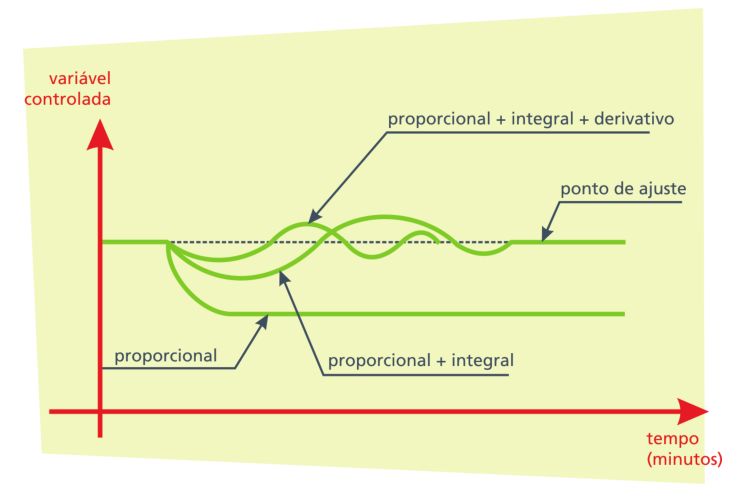
\includegraphics[width=1\linewidth]{Figuras/Ch13/fig1}
\end{frame}


\begin{frame}{Controladores PID}
	\begin{block}{Efeitos na resposta de um controle para as ações P, I e D}
		\resizebox{\textwidth}{!}{
			\begin{tabular}{ccccc}
				\toprule
				\thead{\normalsize Resposta \\\normalsize controle} & \thead{\normalsize Tempo de subida} & \thead{\normalsize \textit{Overshoot}} & \thead{\normalsize Tempo de \\\normalsize estabilização} & \thead{\normalsize Erro no regime \\\normalsize estacionário}\\ \midrule
				P & Diminui & Aumenta & Não altera & \makecell{Diminui, mas \\não elimina} \\[1em]
				I & Diminui & Aumenta & Aumenta & Elimina \\[0.5em]
				D & Não altera & Diminui & Diminui & Não altera \\ \bottomrule
		\end{tabular}}
	\end{block}
\end{frame}


\begin{frame}{Controladores PID}
	
	\centering
	
	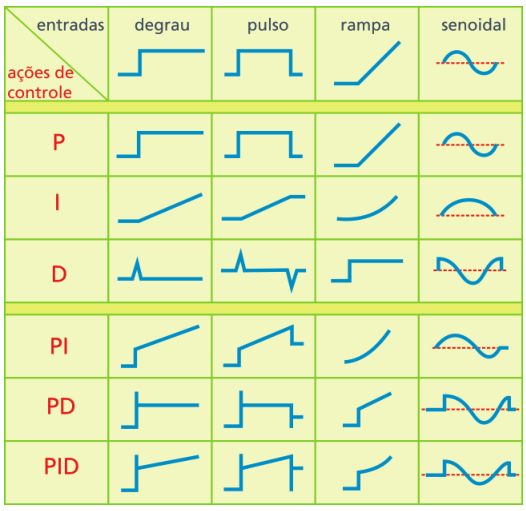
\includegraphics[height=0.9\textheight]{Figuras/Ch13/fig2}
\end{frame}


\begin{frame}{Controladores PID}
	\begin{block}{Formulação matemática}
		\begin{itemize}
			\item Assim como os controladores vistos anteriormente, conseguimos a equação do PID \textbf{somando as equações de suas componentes individuais}, no caso
			\[ VM=C_{p}+C_{i}+C_{d} \]
			expandindo a equação, temos
			\[ VM(t)=K_p\cdot E(t)+K_i\cdot \int_{0}^{t}E(\tau)\dif \tau +K_d\cdot\diff{}{t}\sbr{E(t)} \]
		\end{itemize}
	\end{block}
\end{frame}


\begin{frame}{Controladores PID}
	\begin{block}{Formulação matemática}
		\begin{itemize}
			\item Uma forma \textbf{alternativa} da equação, utilizando os \textbf{tempos integral} e \textbf{derivativo} ($ T_i $ e $ T_d $, respectivamente), segue abaixo:
			\[ VM(t)=K_p\left(E(t)+\dfrac{1}{T_i}\cdot \int_{0}^{t}E(\tau)\dif \tau +T_d\cdot\diff{}{t}\sbr{E(t)} \right) \]
			onde $ K_i=\dfrac{K_p}{T_i} $ e $ K_d=K_p\cdot T_d $
		\end{itemize}
	\end{block}
\end{frame}


\begin{frame}{Controladores PID}
	\centering
	\scalebox{0.75}{
		\deftkzbds
		\begin{tikzpicture}[auto, node distance=1cm,>=Latex]
		\node[input] (in) {};
		\node[sum,right=1.5cm of in] (sum1) {\Large $ + $};
		\coordinate[right=0.75cm of sum1] (p);
		\node[block, right=2cm of sum1] (Cp) {Proporcional};
		\node[block, above=of Cp] (Ci) {Integral};
		\node[block, below=of Cp] (Cd) {Derivativo};			
		\node[sum,right=of Cp] (sum2) {\Large $ + $};
		\node[block, right=of sum2] (P) {Processo};
		\coordinate[right=of P] (mid);
		\node[output,right=of mid] (out) {};
		\node[block,below=3cm of sum2] (S) {Sensor};
		
		\draw[->] (in) -- node[above,midway] {Entrada} (sum1);
		\draw[->] (sum1) -- (Cp);
		\draw[->] (p) |- (Ci);
		\draw[->] (p) |- (Cd);
		\draw[->] (Cp) -- (sum2);
		\draw[->] (Ci) -| (sum2);
		\draw[->] (Cd) -| (sum2);
		\draw[->] (sum2) -- (P);
		\draw[->] (mid) |- (S);
		\draw[->] (S) -| node[pos=0.98, xshift=15pt] {$-$} node[pos=1.12, xshift=-4pt] {$+$} (sum1);
		\draw[->] (P) -- (out) node[above,near end] {Saída};
		\end{tikzpicture}}
	
	\bigskip
	
	Diagrama de blocos
\end{frame}


\begin{frame}{Controladores PID}
	\begin{block}{Exemplo \#01}
		Um \textbf{controlador PID} pode ser utilizado em situações que requeiram \textbf{balanço}, por exemplo, num sistema conhecido como \textbf{``bola-barra''}:
		\begin{itemize}
			\item Uma bola deve permanecer em \textbf{equilíbrio} em \textbf{algum ponto} da barra, sem rolar para nenhum lado.
			\item Para isso dispomos de um \textbf{sensor} que deverá medir o \textbf{deslocamento} da bola no eixo da barra, um \textbf{motor} que pode \textbf{virar} a barra e um \textbf{controlador}, que pode ser um Arduino ou um PC, por exemplo.
			\item Para configurar nosso sistema bola-barra, podemos começar com a componente \textbf{proporcional}, que executará \textbf{o bruto dos movimentos no sistema}.
			\item Para \textbf{configurar os parâmetros} (ganhos) de cada componente utilizamos o conceito de \textbf{sintonia}, que será discutido em profundidade mais à frente.
		\end{itemize}
	\end{block}
\end{frame}


\begin{frame}{Controladores PID}
	
\centering
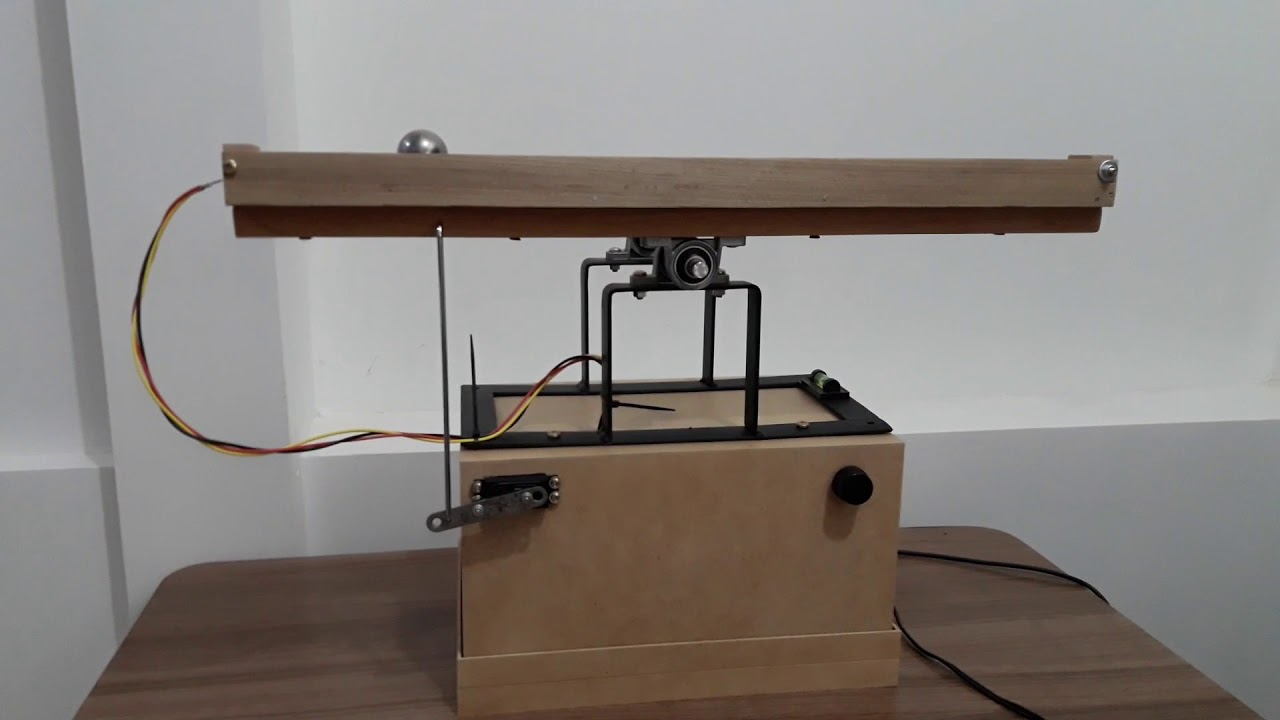
\includegraphics[width=0.9\linewidth]{Figuras/Ch13/fig3}

\end{frame}


\begin{frame}{Controladores PID}
	\begin{block}{Exemplo \#01}
		A componente \textbf{proporcional}, sozinha, fará o sistema \textbf{oscilar}:
		\begin{itemize}
			\item Se as oscilações forem \textbf{muito longas}, a bola pode \textbf{cair da barra}, portanto, as oscilações devem ser \textbf{o mais curtas quanto possível}.
		\end{itemize}
		A partir disso podemos definir a componente \textbf{derivativa}, que deve levar a bola ao \textbf{equilíbrio}:
		\begin{itemize}
			\item Se a componente derivativa for \textbf{muito grande}, a bola ficará em equilíbrio em, virtualmente, \textbf{qualquer parte da barra} (correções muito rápidas), portanto, a componente derivativa deve ter o \textbf{menor ganho possível} para levar a bola à estabilidade.
		\end{itemize}
		
		\begin{itemize}
			\item Por fim, a componente \textbf{integral} deve corrigir qualquer \textbf{erro de \textit{offset}}, presente devido a \textbf{incapacidade} da componente \textbf{proporcional} corrigir erros dentro de uma \textbf{amplitude mínima}, incapaz de vencer as \textbf{resistências internas} ao sistema (atrito, corrente mínima do motor...).
		\end{itemize}
	\end{block}
\end{frame}


\begin{frame}{Controladores PID}
	\begin{block}{Exemplo \#01}
		\begin{itemize}
			\item Podemos formular esse controlador matematicamente utilizando a equação apresentada anteriormente:
			\[ VM(t)=K_p\cdot E(t)+K_i\cdot \int_{0}^{t}E(\tau)\dif \tau +K_d\cdot\diff{}{t}\sbr{E(t)} \]
			\item Sendo o erro $ E(t)=-t^{2}+t $ e os ganhos escolhidos $ K_p=8, K_d=3100, K_i=\num{0.2} $, temos:
			\begin{align*}
				C_p	&=K_p\cdot E(t)\\
					&=8\cdot\del{-t^{2}+t}\\
					&=-8t^{2}+8t
			\end{align*}
		\end{itemize}
	\end{block}
\end{frame}


\begin{frame}{Controladores PID}
	\begin{block}{Exemplo \#01}
		\begin{align*}
			C_d	&=K_d\cdot\diff{}{t}\sbr{E(t)}\\
			&=3100\cdot\diff{}{t}\sbr{-t^{2}+t}\\
			&=3100\cdot\del{-2t}\\
			&=-6200t
		\end{align*}
	\end{block}
\end{frame}


\begin{frame}{Controladores PID}
	\begin{block}{Exemplo \#01}
		\begin{align*}
		C_i	&=K_i\cdot \int_{0}^{t}E(\tau)\dif \tau\\
		&=\num{0.2}\cdot \int_{0}^{t}-\tau^{2}+\tau\dif \tau\\
		&=\num{0.2}\cdot \eval{\del{-\dfrac{1}{3}\tau^{3}+\dfrac{1}{2}\tau^{2}}}_{0}^{t}\\
		&=\num{0.2}\cdot\del{-\dfrac{1}{3}t^{3}+\dfrac{1}{2}t^{2}-\del{\cancel{-\dfrac{1}{3}\cdot0^{3}}+\cancel{\dfrac{1}{2}\cdot0^{2}}}}\\
		&=\num{0.2}\cdot\del{-\dfrac{1}{3}t^{3}+\dfrac{1}{2}t^{2}}\\
		&=-\num{0.067}t^{3}+\num{0.1}t^{2}
		\end{align*}
	\end{block}
\end{frame}


\begin{frame}{Controladores PID}
	\begin{block}{Exemplo \#01}
		\begin{itemize}
			\item Juntando tudo, temos:
			\begin{align*}
				VM(t)&=-8t^{2}+8t-\num{0.067}t^{3}+\num{0.1}t^{2}-6200t\\
					&=-\num{0.067}t^{3}-\num{7.9}t^{2}-6192t
			\end{align*}
		\end{itemize}
	\end{block}
\end{frame}


\begin{frame}{Controladores PID}
	\begin{block}{Exemplo \#01}
		\begin{itemize}
			\item O sistema bola-barra pode ser utilizado em \textbf{duas dimensões} com uma placa de apoio ao invés de uma barra.
			\item Podemos ver a superfície da placa como um \textbf{gráfico com dois eixos}, onde cada um sofre o \textbf{mesmo controle} da barra no exemplo.
		\end{itemize}
	\end{block}
	
	\centering
	
	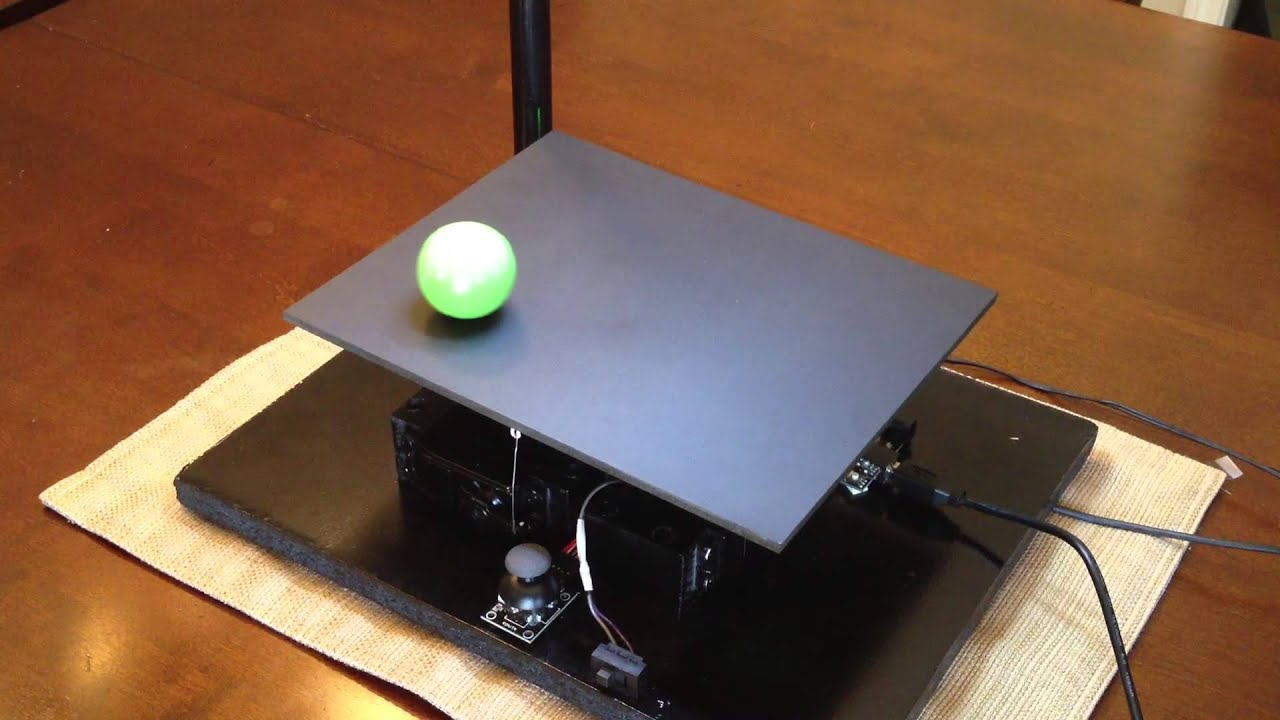
\includegraphics[width=0.7\linewidth]{Figuras/Ch13/fig5}
\end{frame}


\begin{frame}{Controladores PID}
	\begin{block}{Exemplo \#02}
		\begin{itemize}
			\item Um outro exemplo, também relacionado à balanço, porém mais interessante, é o de um \textbf{eixo com rotores}.
			\item Assim como no sistema bola-barra, podemos usar um \textbf{controlador PID} para fazer o sistema ficar em \textbf{equilíbrio}.
		\end{itemize}
	\end{block}

	\medskip

	\centering
	
	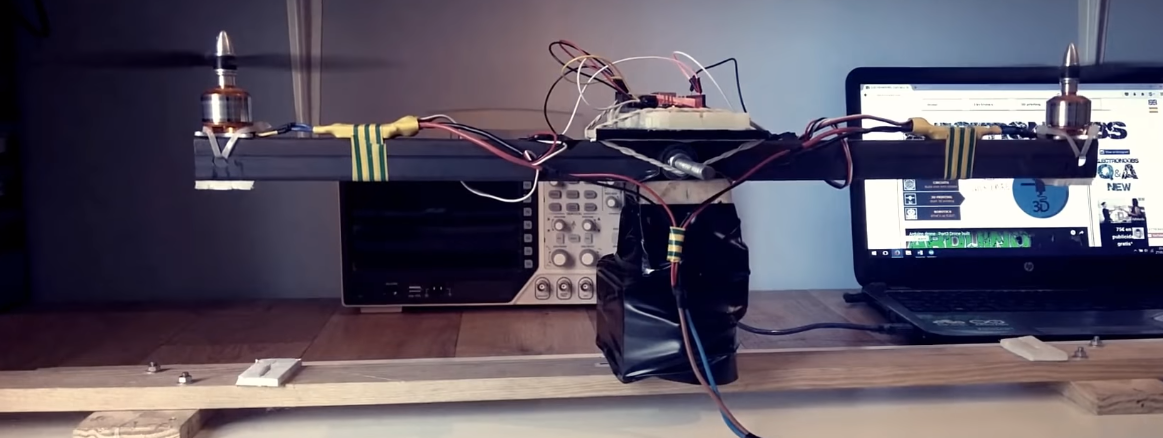
\includegraphics[width=0.9\linewidth]{Figuras/Ch13/fig4}
\end{frame}


\begin{frame}{Controladores PID}
	\begin{block}{Exemplo \#02}
		\begin{itemize}
			\item Similarmente, podemos encontrar a equação deste controlador com a fórmula
			\[ VM(t)=K_p\cdot E(t)+K_i\cdot \int_{0}^{t}E(\tau)\dif \tau +K_d\cdot\diff{}{t}\sbr{E(t)} \]
			\item Sendo o erro $ E(t)=4t^{3}-2t-\num{0.5} $ e os ganhos escolhidos $ K_p=3, K_d=2, K_i=\num{0.048} $, temos:
			\begin{align*}
			C_p	&=K_p\cdot E(t)\\
			&=3\cdot\del{4t^{3}-2t-\num{0.5}}\\
			&=12t^{3}-6t-\num{1.5}
			\end{align*}
		\end{itemize}
	\end{block}
\end{frame}


\begin{frame}{Controladores PID}
	\begin{block}{Exemplo \#02}
		\begin{align*}
		C_d	&=K_d\cdot\diff{}{t}\sbr{E(t)}\\
		&=2\cdot\diff{}{t}\sbr{4t^{3}-2t-\num{0.5}}\\
		&=2\cdot\del{12t^{2}-2}\\
		&=24t^{2}-4
		\end{align*}
	\end{block}
\end{frame}


\begin{frame}{Controladores PID}
	\begin{block}{Exemplo \#02}
		\begin{align*}
		C_i	&=K_i\cdot \int_{0}^{t}E(\tau)\dif \tau\\
		&=\num{0.048}\cdot \int_{0}^{t}4\tau^{3}-2\tau-\num{0.5}\dif \tau\\
		&=\num{0.048}\cdot \eval{\del{\tau^{4}-\tau^{2}-\num{0.5}\tau}}_{0}^{t}\\
		&=\num{0.048}\cdot\del{t^{4}-t^{2}-0.5t-\del{\cancel{0^{4}}-\cancel{0^{2}}-\cancel{\num{0.5}\cdot0}}}\\
		&=\num{0.048}\cdot\del{t^{4}-t^{2}-\num{0.5}t}\\
		&=\num{0.048}t^{4}-\num{0.048}t^{2}-\num{0.024}t
		\end{align*}
	\end{block}
\end{frame}


\begin{frame}{Controladores PID}
	\begin{block}{Exemplo \#02}
		\begin{itemize}
			\item Juntando tudo, temos:
			\begin{align*}
			VM(t)&=12t^{3}-6t-\num{1.5}+\num{0.048}t^{4}-\num{0.048}t^{2}-\num{0.024}t+24t^{2}-4\\
			&=\num{0.048}t^{4}+12t^{3}+\num{23.952}t^{2}-\num{6.024}t-\num{5.5}
			\end{align*}
		\end{itemize}
	\end{block}
\end{frame}


\begin{frame}{Controladores PID}
	\begin{block}{Exemplo \#02}
		\begin{itemize}
			\item O equivalente desse sistema em duas dimensões é um \textbf{drone}.
		\end{itemize}
	\end{block}
	
	\medskip
	
	\centering
	
	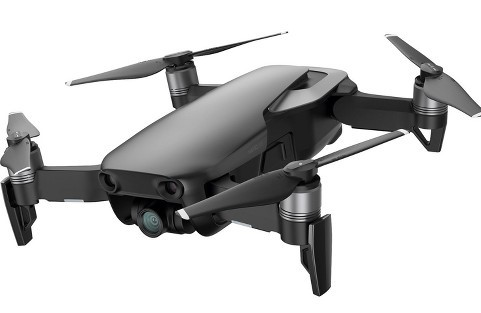
\includegraphics[width=0.8\linewidth]{Figuras/Ch13/fig6}
\end{frame}


\begin{frame}{Controladores PID}
	\begin{block}{Exemplo \#03}
		\begin{itemize}
			\item Podemos utilizar um controlador PID para o controle da \textbf{temperatura}, por exemplo, num laboratório que precisa \textbf{conservar amostras} a uma \textbf{temperatura específica}.
		\end{itemize}
	\end{block}
	
	\medskip
	
	\centering
	
	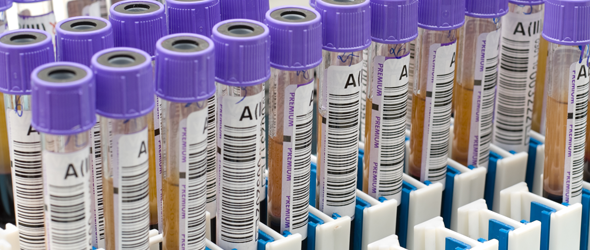
\includegraphics[width=0.9\linewidth]{Figuras/Ch13/fig7}
\end{frame}


\begin{frame}{Controladores PID}
	\begin{block}{Exemplo \#03}
		\begin{itemize}
			\item Utilizando a fórmula
			\[ VM(t)=K_p\cdot\left( E(t)+\dfrac{1}{T_i}\cdot \int_{0}^{t}E(\tau)\dif \tau +T_d\cdot\diff{}{t}\sbr{E(t)}\right) \]
			\item Sendo o erro $ E(t)=6t-10, BP=50\%, T_i=\SI{3}{\second}, T_d=\SI{2}{\second} $ , temos:
			\begin{align*}
				BP	&=\dfrac{100\%}{K_p}\Rightarrow\\
				K_p	&=\dfrac{100\%}{BP}\\
					&=\dfrac{100\%}{50\%}\\
					&=2
			\end{align*}
		\end{itemize}
	\end{block}
\end{frame}


\begin{frame}{Controladores PID}
	\begin{block}{Exemplo \#03}
		\begin{align*}
			\diff{}{t}\sbr{E(t)}&=\diff{}{t}\sbr{6t-10}=6\\[0.5em]
			\int_{0}^{t}E(\tau)\dif\tau	&=\int_{0}^{t}6\tau-10\dif\tau\\
										&=\eval{\del{\dfrac{6}{2}\tau^{2}-10\tau}}_{0}^{t}\\
										&=\del{3t^{2}-10t-\del{\cancel{3\cdot0^{2}}-\cancel{10\cdot0}}}\\
										&=3t^{2}-10t
		\end{align*}
	\end{block}
\end{frame}


\begin{frame}{Controladores PID}
	\begin{block}{Exemplo \#03}
		\begin{itemize}
			\item Juntando tudo, temos:
			\begin{align*}
				VM(t)&=K_p\cdot\left( E(t)+\dfrac{1}{T_i}\cdot \int_{0}^{t}E(\tau)\dif \tau +T_d\cdot\diff{}{t}\sbr{E(t)}\right)\\
					&=2\cdot\left( \del{6t-10}+\dfrac{1}{3}\cdot\del{3t^{2}-10t}+2\cdot\del{6} \right)\\
					&=2\cdot\left( 6t-10+t^{2}-\num{3.33}t+12 \right)\\
					&=2\cdot\left( t^{2}+\num{2.67}t+2 \right)\\
					&=2t^{2}+\num{5.34}t+4
			\end{align*}
		\end{itemize}
	\end{block}
\end{frame}


\frame{
	\frametitle{Exercícios}
	\begin{block}{}
		01. Desenvolva as formulações matemáticas dados:
		
		\medskip
		
		\begin{minipage}{0.49\linewidth}
			(a) \begin{align*}
			E(t)&=2t^{3}-5t+12\\
			BP&=40\%\\
			T_i&=\SI{3}{\second}\\
			T_d&=\SI{2}{\second}
			\end{align*}
			
			\vspace{0.5cm}
			
			(c) \begin{align*}
			E(t)&=2t^{3}+5t^{2}-\num{0.2}\\
			K_p&=32\\
			K_i&=\num{0.024}\\
			K_d&=1
			\end{align*}
		\end{minipage}
		\hfill
		\begin{minipage}{0.49\linewidth}
			(b) \begin{align*}
			E(t)&=t^{3}\\
			K_i&=12\\
			T_i&=\SI{0.03}{\second}\\
			T_d&=\SI{4}{\second}
			\end{align*}
			
			\vspace{0.5cm}
			
			(d) \begin{align*}
			E(t)&=\del{t+5}^{2}\\
			BP&=120\%\\
			T_i&=\SI{5}{\second}\\
			T_d&=\SI{3}{\second}
			\end{align*}
		\end{minipage}
	\end{block}
}


\section*{Referências}
\frame{
	\frametitle{Referências e Exercícios Complementares}
	\begin{itemize}
		\item BAYER, Fernando Mariano; ARAÚJO, Olinto César Bassi de. Controle Automático de Processos, 3 ed. UFSM : Colégio Técnico Industrial de Santa Maria, 2011.
	\end{itemize}
	%\centering{\alert{Página 546 - \textbf{Capítulo 6}}} \\
	%\centering{\alert{Lista de exercícios 01}}
}